 \section{Scope of study}

Innovation encompasses the invention, development, and implementation of new ideas \citep{garud2013perspectives,bessant2013innovation}. Business enterprises are increasingly obliged to engage in continuous innovation in order to remain competitive in an ever-demanding and rapidly evolving knowledge-based economy \citep{lubit2001keys,urbancova2013competitive,lee2019does,jackson2020fostering}. However, business enterprises also struggle to keep pace with technological advances and cannot rely solely upon their internal knowledge for innovation \citep{nunes2020managing}. Unsurprisingly, many business enterprises are turning to open innovation as a competitive strategy \citep{stanko2017under,lee2019does}. With open innovation, the innovation process relies heavily on accessing, absorbing, and harnessing knowledge across organisational boundaries \citep{chesbrough2017future}. \medskip

Little is known about the role of tacit knowledge in open innovation, which is remarkable, considering tacit knowledge guides the learning and thought processes that produce novel ideas \citep{leonard1998role}. Knowledge exists of a spectrum from entirely tacit to completely explicit \citep{leonard1998role}. Thus, any knowledge that crosses organisational boundaries is likely to have a tacit component to it, more so if the knowledge is very complex \citep{seidler2008use,szulanski2016overcoming}. Despite the importance of tacit knowledge for innovation, it has received scant attention in the open innovation literature (see Figure \ref{fig:biblio}). \medskip

This thesis attempts to fill this gap by examining tacit knowledge sharing in three open innovation partnerships. Because tacit knowledge is shared primarily as an act of volition or free-will \citep{polanyi1966tacit}, attention focuses on how human agency and organisational structures affect tacit knowledge sharing. \medskip

\begin{figure}[p]
\centering
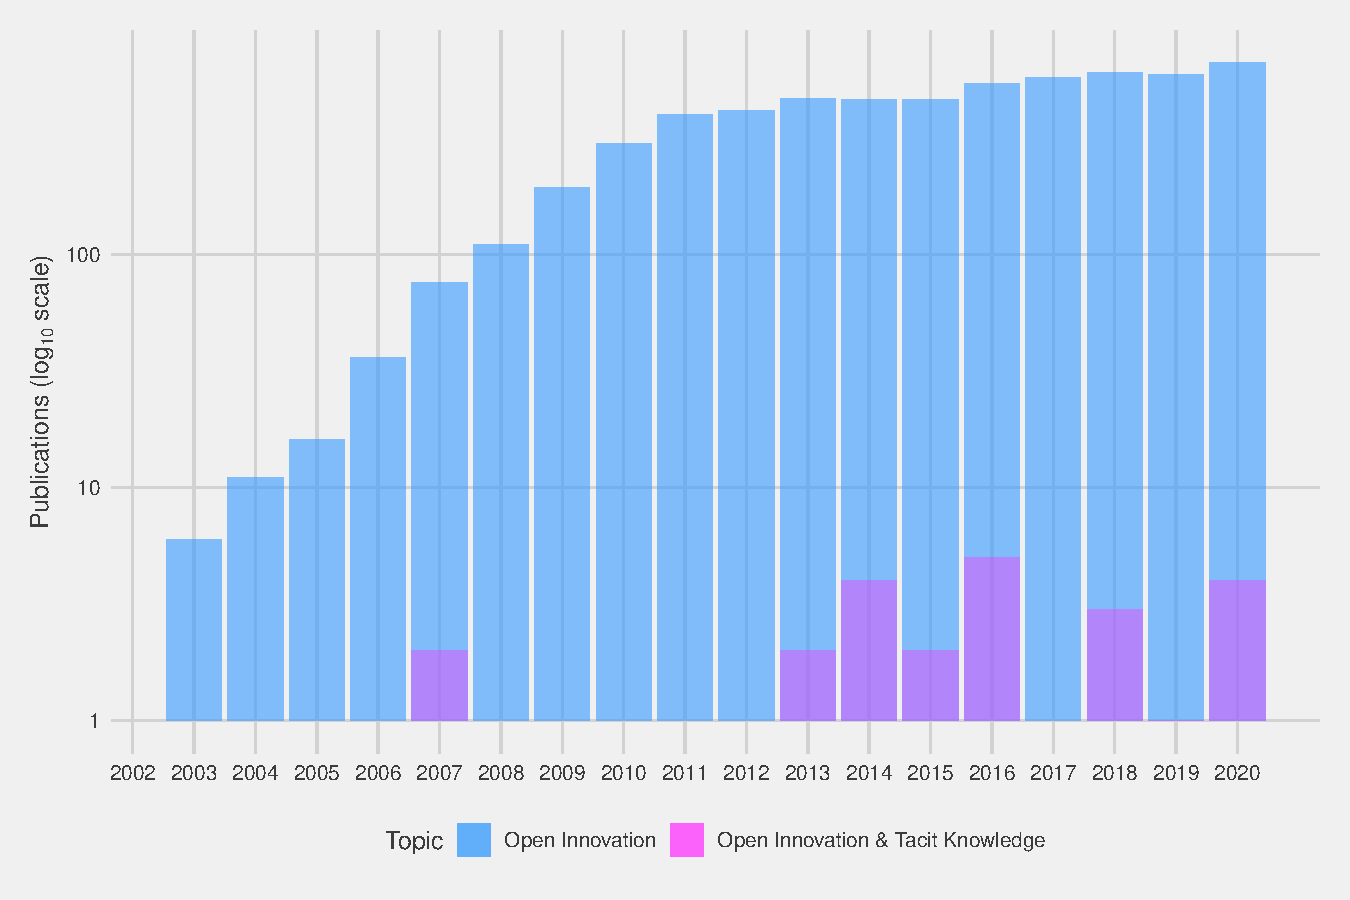
\includegraphics[width=0.9\linewidth]{Images/tk_oi.pdf}
\caption[Articles published each year on open innovation]{Articles published each year on open innovation with the relative proportion of articles referencing tacit knowledge. Few articles address tacit knowledge directly. Data from Scopus (search queries: TITLE-ABS-KEY ("open innovation") and TITLE-ABS-KEY ("tacit knowledge"  AND  "open innovation")).}
\label{fig:biblio}
\end{figure}

\section{Background}

\subsection{Trend towards open innovation} \label{sss:oi}

Proponents of the resource-based view of the firm argue that competitive advantage stems from the application of tangible and intangible resources available to it \citep{wernerfelt1984resource,peteraf1993cornerstones}. The extent to which a firm can sustain competitive advantage depends on how valuable, rare, inimitable, and non-substitutable its resources are \citep{barney1991firm}. Because knowledge fuels innovation, it is arguably the most critical resource for a firm competing in a fast-moving and technology-driven economy \citep{grant1996toward,urbancova2013competitive}. However, the proliferation of increasingly specialised knowledge means that firms are finding it harder to compete using only their internal knowledge resources \citep{chesbrough2009open,enkel2009open}. Many firms are turning to open innovation as a competitive strategy \citep{stanko2017under,lee2019does}. \medskip

Open innovation is a distributed innovation process involving purposely managed knowledge flows across organisational boundaries, using mechanisms in line with the firm's business model \citep{chesbrough2014explicating}. The business model helps a firm decide what external knowledge can fuel innovation and which knowledge to release to other organisations \citep{chesbrough2017future}. Key benefits of open innovation include timely access to new knowledge or technology, sharing of risk, reduced costs of development, better customer acceptance of products or services, and enhanced ability to innovate continuously \citep{ye2013exploring}. \medskip
 
 Open innovation can be described in terms of \enquote{inbound}, \enquote{outbound} and \enquote{coupled} innovation processes \citep{gassmann2004towards}. Inbound open innovation enriches a firm's knowledge base through integrating suppliers, customers and other external actors \citep{xu2013inbound}, whereas outbound open innovation refers to the commercial exploitation of knowledge developed in-house \citep{de2016knowledge}. Coupled open innovation focuses on strategic partnerships that encompass both inbound and outbound innovation processes \citep{spithoven2013open}. Figure \ref{fig:oi_funnel} illustrates how these processes may work in practice. \medskip
 
\begin{figure}[p]
\centering
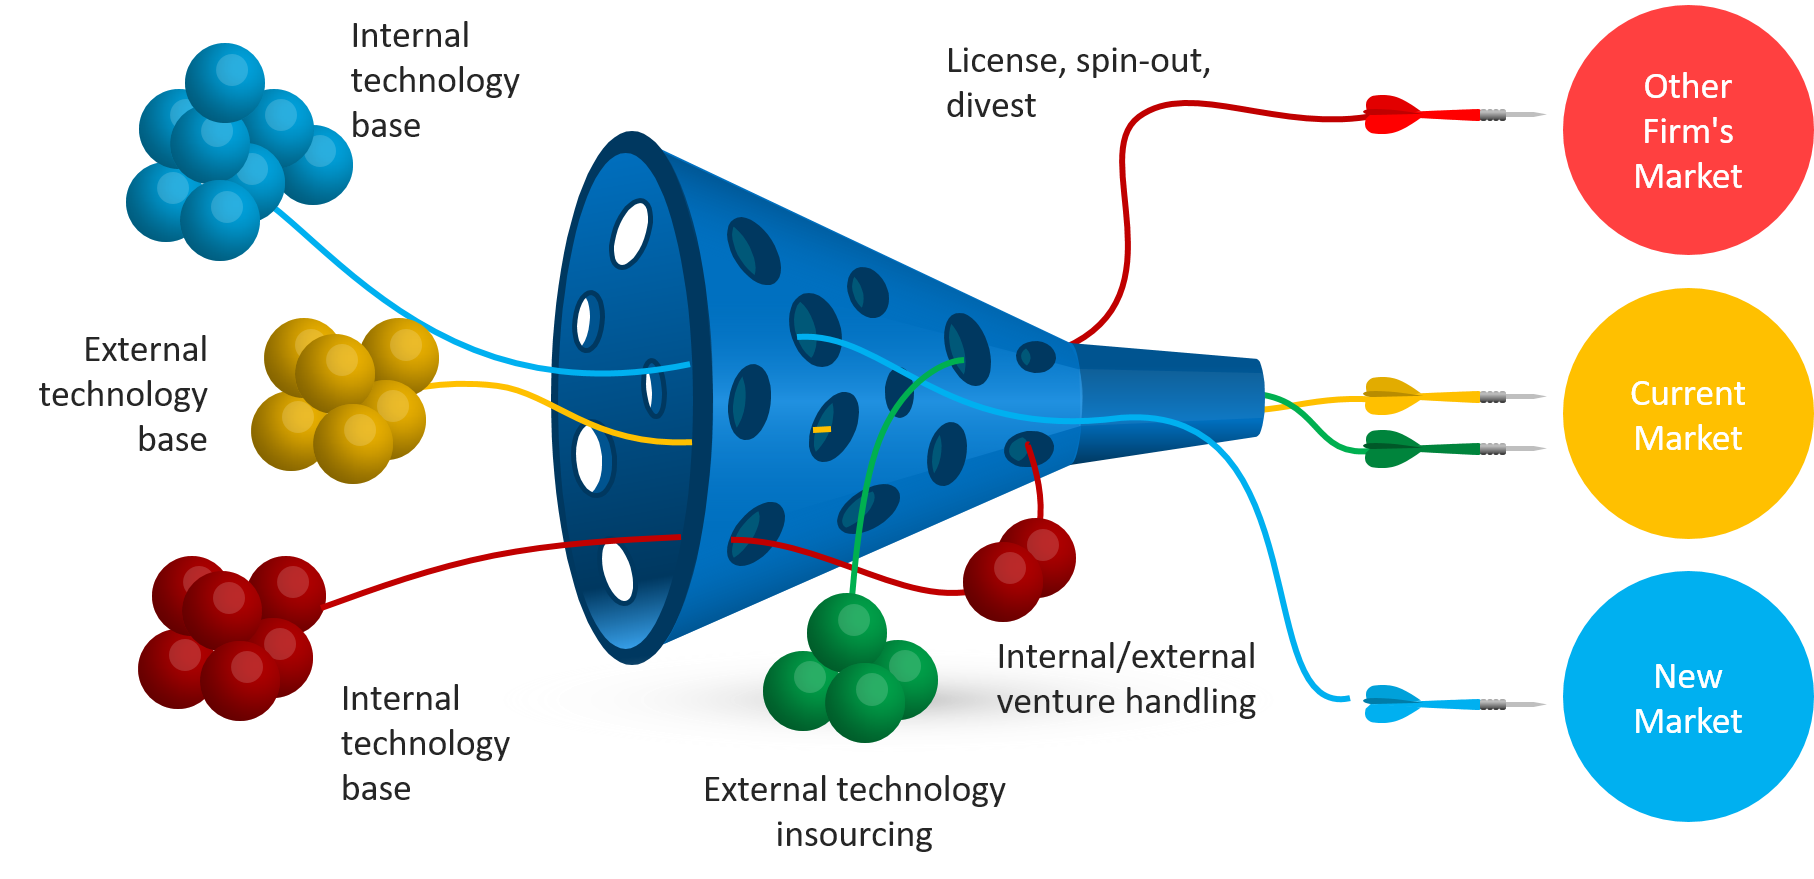
\includegraphics[width=0.9\linewidth]{Images/oi_funnel.png}
\caption[Open innovation funnel]{Open innovation funnel illustrating inbound, outbound, and coupled innovation processes. Open innovation presents multiple pathways for generating value from knowledge. How easily knowledge is able to flow across organisational boundaries depends on the strength of inter-organisational relationships and the absorptive and desorptive capacity of partners \citep{lichtenthaler2010technology, kokshagina2017fast,bigliardi2021past}.} 
\label{fig:oi_funnel}
\end{figure}

With open innovation, the locus of knowledge creation does not necessarily correspond to the locus of innovation \citep{gassmann2004towards}. In the case of inbound open innovation, the locus of innovation is inside the firm receiving new external knowledge. With outbound open innovation, the locus of innovation is external to the firm providing knowledge. The locus of innovation with coupled innovation straddles firm boundaries. Likewise, the locus of exploitation (i.e. the application of knowledge for commercial benefit) can also be different to the locus of innovation. A firm may come up with an innovative solution to a problem through inbound open innovation, but use outbound open innovation for commercial exploitation by a third-party \citep{gassmann2004towards}. A good example is Nokia Corporation. The Finnish company was a market leader in mobile telephone handsets but became sidelined when US competitors introduced more capable \textquote{smart phones} into the market. Nokia has pivoted, using its know-how in mobile telephony to provide novel cellular network solutions (e.g. fifth-generation cellular network technology (5G) and services for the Internet of Things (IoT)) to service providers (outbound open innovation). Nokia has a strategic partnership with US-based Bell Laboratories to develop next-generation communications technologies (inbound/coupled open innovation)\footnote{\url{https://www.nokia.com/system/files/2020-03/Nokia\%20Form\%2020F\%202019_0.pdf}}.  
 
\subsection{Key capabilities for open innovation}

Different capabilities are required for inbound, outbound, and coupled open innovation. Firms pursuing inbound open innovation, for instance, need absorptive capacity to make sense of, and exploit, unfamiliar external knowledge  \citep{vanhaverbeke2007,connectingkokshagina2017fast,bigliardi2021past}. Relative differences in absorptive capacity between open innovation partners can impede knowledge integration, contribute to power imbalances, and undermine alliance performance, all of which can result in sub-optimal open innovation outcomes \citep{lane1998relative,vanhaverbeke2007connecting,zobel2016benefiting,tell2017managing}. Overcoming relative differences in absorptive capacity is crucial for successful open innovation and requires partners to have a strong learning orientation to help align thinking and reduce differences in understanding between them  \citep{nooteboom2000learning,sun2010examination,de2016knowledge}. \medskip

Firms wanting to exploit their internally developed knowledge through outbound open innovation require \enquote{desorptive capacity} to identify and act on knowledge transfer opportunities \citep{lichtenthaler2010technology}. This includes having appropriate mechanisms for managing and leveraging intellectual property \citep{chesbrough2012open,denford2018absorption}. Absorptive and desorptive capacity can be seen as two sides of the same coin, i.e. they are pull and push factors governing knowledge transfer processes \citep{dell2015absorptive}. \medskip

Another important capability needed for open innovation is the ability to develop and maintain strong and productive inter-organisational networks \citep{chesbrough2012open,yun2016network,schepis2021facilitating}. Such an ability requires people who can operate effectively across organisational boundaries \citep{tushman1981boundary,meyer2010rise,quintane2016brokers}. Effective boundary spanners are not only able to broker new relations that extend or widen existing inter-organisational knowledge networks, but also play a key role in building trust and reducing the cognitive distance between open innovation partners \citep{fleming2007brokerage,goffin2010managing,renzl2008trust,sankowska2013relationships,kucharska2016trust}. 

\subsection{Role of tacit knowledge in open innovation}

\citet{kreutz2014catalyzing} define tacit knowledge as the \enquote{unwritten, unspoken, and hidden vast storehouse of knowledge held by practically every normal human being, based on his or her emotions, experiences, insights, intuition, observations, and internalised information}. They go on to state that \enquote{like the submerged part of an iceberg, tacit knowledge constitutes the bulk of what one knows, and forms the underlying framework that makes explicit knowledge possible}. Tacit knowledge provides important context for making sense of explicit knowledge, especially if such knowledge is highly specialised or complex \citep{von1994sticky,szulanski1996exploring,leonard1998role,seidler2008use}. \medskip

The leading edge of the firm’s learning often is found in the tacit knowledge of its employees \citep{horvath2000working}. Indeed, tacit knowledge is strongly implicated in innovation as it guides the learning and thought processes that produce novel ideas \citep{leonard1998role,amar2008descriptive,leonard2014knowledge}. Tacit knowledge helps bridge cognitive gaps and thus underpins a firm's absorptive capacity \citep{thomas2021tacit}. Because tacit knowledge is embodied in people and embedded in the things they create, it helps a firm resist imitation by competitors \citep{horvath2000working}. \medskip

Not only is tacit knowledge deeply rooted in personal experience, it is also inculcated in group practice and culture, usually in the form of unwritten rules and procedures \citep{nonaka1995knowledge,howells1996tacit}. Some argue that tacit knowledge is a defining feature of the various sub-cultures that exist within a firm \citep[e.g.][]{smith2001role,munoz2015tacit}. Mobilising tacit knowledge in open innovation is challenging because individuals or groups are either unaware of the tacit dimension of their knowledge, or are unable to express what they know \citep{polanyi1966tacit}. Many firms do not appreciate the depth of their knowledge base and lack processes to unlock the potential value of tacit knowledge embodied in the minds and actions of employees \citep{nonaka1994dynamic,howells1996tacit,horvath2000working}. \medskip

Moreover, people cannot be coerced to share their tacit knowledge. Agency lies at the heart of tacit knowledge sharing \citep{polanyi1966tacit, emirbayer1994network}. Finding the right balance between structure and agency is a challenge in open innovation \citep{longo2017struggling}. Too much structure may inhibit participants' willingness to share tacit knowledge or contribute ideas. Conversely, too little structure can make goals less clear, leading to unsatisfactory open innovation outcomes \citep{davis2010agency,lam2014tacit}. \medskip

Adding to the challenge is the notion that tacit knowledge is not transferred but rather interpreted within a specific context \citep{nonaka1995knowledge,duguid2005art,marabelli2014knowing,zhang2020extended}. Face-to-face social interaction is key because it allows immediate feedback to confirm understanding and correct any misinterpretations \citep{haldin2000difficulties,gertler2003tacit,koskinen2003tacit}. While advances in information technology (e.g. e-mail, instant messaging, video-conferencing, web-based collaboration platforms, and augmented or virtual reality) make it easier for dispersed team members to communicate with each other, much of this information technology is limited in how it can facilitate tacit knowledge exchange. Limited face-to-face interaction may negatively impact knowledge sharing and idea generation in open innovation \citep{johannessen2001mismanagement}. Neglecting the tacit dimension of inter-organisational knowledge exchanges may result in sub-optimal, or even worse, failed open innovation outcomes. 

\section{Research context}

\subsection{A network perspective of open innovation}

Since open innovation involves multiple organisations exchanging knowledge with one another, this study conceptualises an open innovation partnership as a temporary knowledge network, one that is deliberately set up to achieve a specific innovation outcome within a market-relevant time frame \citep{perez2013temporary,cococcioni2014exploring,terhorst2018tacit}. Knowledge networks represent collections of individuals and teams that come together across organisational, spatial and disciplinary boundaries to create, share or apply a body of knowledge \citep{pugh2013designing}. Though tacit knowledge has a key role to play in transferring specialised or complex knowledge \citep{davenport1998working,sternberg1999tacit,johnson2002all,endres2007tacit,tell2017managing}, the extent to which it helps bridge cognitive gaps and stimulate idea generation is poorly understood. As tacit knowledge exchange is a socially intensive process, there is merit in using social network analysis to assess tacit knowledge flows in open innovation \citep{leonard1998role,busch2000graphically,zhu2007social}. Such analysis can provide useful insights into both endogenous (inherent) and exogenous (environmental) factors that influence tacit knowledge transfer processes \citep{kolleck2013social,tortoriello2015social}. 

\subsection{Exploring motivational factors}

Tacit knowledge requires significantly more effort to communicate than explicit knowledge. It requires commitment to learn from, or to teach, others. In other words, individuals have to be sufficiently motivated to seek out and share tacit knowledge \citep{leonard1998role}. This includes becoming more aware of the tacit dimension of knowledge and making an effort to understand what this means in terms of innovation and absorptive capacity. Motivation is a theoretical construct used to explain individual behaviour. More specifically, a motive is what prompts a person to act in a specific way or develop an inclination towards a particular behaviour \citep{pardee1990motivation}. Past studies show a significant and positive relation between an individual's level of intrinsic motivation and the amount of tacit knowledge they share \citep[e.g.][]{osterloh2000motivation,kaser2001knowledge,smith2001role}. Intrinsic motivation is about engaging in activities because these are enjoyable or personally meaningful \citep{ryan2000intrinsic}. Although these studies highlight the importance of personal motivation, the psychosocial processes underpinning tacit knowledge exchange in open innovation are not well understood. Open innovation is unlikely to succeed without highly motivated individuals.

\subsection{Unpacking power-relations} 

Though it is often stated that \enquote{knowledge is power}, not much is written about power and power-relations in the knowledge management literature \citep{haugaard2012rethinking}. The current literature on power is dominated by two contrasting views of power, namely \textquote{power as domination}, also referred to as \textquote{power-over}, and \textquote{power as empowerment}, often characterised as \textquote{power-to} \citep{haugaard2012rethinking}.  People accumulate tacit knowledge to empower themselves in their quest for competence or self-efficacy \citep{endres2007tacit}. By sharing their tacit knowledge, individuals are essentially empowering others to perform work more independently and confidently \citep{bordum2002tacit,lin2007share}. Some people may be reluctant to share their hard-earned tacit knowledge if they think this will compromise or dis-empower them \citep{schultze2004knowing,singh2019territoriality}. \medskip

The social network perspective, which focuses on relationships between different entities in a given social context,  treats power as inherently relational \citep{ibarra1993power}. As mentioned earlier, knowledge brokers play a vital role in open innovation as they connect individuals, coordinate interactions between partners, and help others make sense of unfamiliar knowledge. Because of their central network position, they can exert considerable influence over knowledge flows \citep{burt1992structural}. By examining brokerage patterns in knowledge networks, one may be able to infer how partners exercise power in open innovation. Analysis of brokerage patterns should reveal which individuals benefit from knowledge exchanges and highlight the most significant brokerage mechanisms at play in an open innovation partnership. 

\section{Thesis objectives}

This thesis employs mixed-method social network analysis to explore tacit knowledge sharing in three open innovation partnerships. Mixed-method social network analysis enables the exploration of network structure while not forsaking the qualitative observations about what is going on within a network, e.g. external social forces, mechanisms and structures that shape tacit knowledge sharing relations \citep{crossley2010social}. Using a mixed methods is fraught because of the complex ontological and epistemological issues involved \citep{giddings2006mixed,mcevoy2006critical}. Consequently, this thesis embraces a critical realist worldview to make sense of data collected under different epistemological assumptions \citep{johnson2004mixed,giddings2006mixed,welch2011theorising}. \medskip

As tacit knowledge sharing is primarily an act of volition or free-will, the thesis considers how agency and structure affect tacit knowledge sharing in open innovation. It addresses the following research question: What does social network analysis reveal about tacit knowledge sharing behaviour in open innovation partnerships? This research question can be broken down into four sub-questions:

\begin{enumerate}
\item What does the structure of tacit knowledge networks reveal about knowledge sharing in open innovation?
\item Does brokerage differ according to the type of knowledge being shared?
\item To what extent does self-determination drive tacit knowledge sharing in open innovation?
\item What does the micro-structure of tacit knowledge networks reveal about trust and power-relations in open innovation partnerships?
\end{enumerate}

\section{Research contribution}

This thesis advances knowledge by providing fresh insight into the role of tacit knowledge in open innovation partnerships. It demonstrated the application of agency theory in an open innovation context and found that self-determination theory can explain tacit knowledge-seeking behaviour in inter-organisational knowledge networks. People who were deeply committed to partnership goals were more likely to exchange know-how, whereas those with superior attitudes or who were close-minded were less likely to exchange know-how. The thesis found that modelling of broker roles provided a more nuanced and precise explanation of the structure of inter-organisational knowledge networks. This should help managers design more effective open innovation partnerships to ensure that complex or specialised (also referred to as \textquote{sticky}) knowledge flows more easily across organisational boundaries. Another contribution of this thesis will be the development and testing of a more robust framework for mixed-method social network analysis that others can use. 

\section{Document structure}

The remainder of this document is organised as follows:

\begin{itemize}[leftmargin=0pt]
    \item[] \textbf{Chapter 2} considers the epistemology of knowledge and what this means in terms of absorptive capacity and knowledge brokerage.
    \item[] \textbf{Chapter 3} reviews key literature on motivation, trust, and power relevant to tacit knowledge sharing. \textbf{Chapters 2} and \textbf{3} present a number of propositions that inform the subsequent mixed-method analysis. The propositions address key aspects of the four research sub-questions. 
    
    \item[] \textbf{Chapter 4} describes the critical realist research methodology underpinning this study. This includes a justification for using mixed-methods and details the quantitative and qualitative procedures used to collect and analyse data.
    \item[] \textbf{Chapter 5} describes and contrasts the three open innovation partnerships investigated in this study.
    \item[] \textbf{Chapter 6} presents the results of the statistical network analysis that examined the role of motivation, trust, and power in tacit and explicit knowledge exchanges, and the significance of different broker roles in each case.
    \item[] \textbf{Chapter 7} presents the results of the qualitative analysis of the semi-structured interviews.
    \item[] \textbf{Chapter 8} discusses the quantitative and qualitative results from a critical realist perspective. 
    \item[] \textbf{Chapter 9} summarises the main findings of this study and reflects on some key lessons learned as this study unfolded. This includes descriptions of the study's limitations and possible avenues for future research. 
\end{itemize}